\documentclass{report}

\input{~/dev/latex/template/preamble.tex}
\input{~/dev/latex/template/macros.tex}

\title{\Huge{}}
\author{\huge{Nathan Warner}}
\date{\huge{}}
\pagestyle{fancy}
\fancyhf{}
\lhead{Warner \thepage}
\rhead{}
% \lhead{\leftmark}
\cfoot{\thepage}
%\setborder
% \usepackage[default]{sourcecodepro}
% \usepackage[T1]{fontenc}

\begin{document}
    % \maketitle
        \begin{titlepage}
       \begin{center}
           \vspace*{1cm}
    
           \textbf{Calculus 2} \\
           Chapter 6
    
           \vspace{0.5cm}
            
                
           \vspace{1.5cm}
    
           \textbf{Nathan Warner}
    
           \vfill
                
                
           \vspace{0.8cm}
         
           
\includegraphics[width=0.4\textwidth]{~/niu/seal.png}
                
           Computer Science \\
           Northern Illinois University\\
           October 27, 2023 \\
           United States\\
           
                
       \end{center}
    \end{titlepage}
    \tableofcontents
    \pagebreak \bigbreak \noindent
    \vspace{2in} \\
    \begin{Huge}
       \textbf{Power Series} 
    \end{Huge}
    \bigbreak \noindent 
    \line(1,0){490}
    \bigbreak \noindent 
    \phantomsection
    \addcontentsline{toc}{section}{6.1 Power Series and Functions}
    \section*{6.1 Power Series and Functions}
    \bigbreak \noindent 
    A power series is a type of series with terms involving a variable. More specifically, if the variable is x, then all the terms of the series involve powers of x. As a result, a power series can be thought of as an infinite polynomial. Power series are used to represent common functions and also to define new functions. In this section we define power series and show how to determine when a power series converges and when it diverges. We also show how to represent certain functions using power series.
    \bigbreak \noindent 
    \phantomsection
    \addcontentsline{toc}{subsection}{Form of a Power Series}
    \subsection*{Form of a Power Series}
    \bigbreak \noindent 
    \begin{definition}
        A series of the form
    \begin{align*}
        \sum_{n=0}^{\infty} c_n x^n &= c_0 + c_1 x + c_2 x^2 + \cdots 
    .\end{align*}
    is a power series centered at \( x = 0 \).
    \bigbreak \noindent 
    A series of the form
    \begin{align*}
        \sum_{n=0}^{\infty} c_n (x - a)^n &= c_0 + c_1 (x - a) + c_2 (x - a)^2 + \cdots 
    .\end{align*}
    is a power series centered at \( x = a \).
    \end{definition}
    
    \bigbreak \noindent 
    To make this definition precise, we stipulate that \( x^0 = 1 \) and \( (x - a)^0 = 1 \) even when \( x = 0 \) and \( x = a \), respectively.
    \bigbreak \noindent 
    The series
    \begin{align*}
        \sum_{n=0}^{\infty} \frac{x^n}{n!} &= 1 + x + \frac{x^2}{2!} + \frac{x^3}{3!} + \cdots
    \end{align*}
    and
    \begin{align*}
        \sum_{n=0}^{\infty} n! x^n &= 1 + x + 2! x^2 + 3! x^3 + \cdots
    \end{align*}
    are both power series centered at \( x = 0 \).
    \bigbreak \noindent 
    The series
    \begin{align*}
        \sum_{n=0}^{\infty} \frac{(x - 2)^n}{(n + 1)3^n} &= 1 + \frac{x - 2}{2 \cdot 3} + \frac{(x - 2)^2}{3 \cdot 3^2} + \frac{(x - 2)^3}{4 \cdot 3^3} + \cdots
    \end{align*}
    is a power series centered at \( x = 2 \).

    \bigbreak \noindent 
    \phantomsection
    \addcontentsline{toc}{subsection}{Convergence of a Power Series}
    \subsection*{Convergence of a Power Series}
    \bigbreak \noindent 
    \begin{thrm}[Convergence of a Power Series]
        Consider the power series \(\sum_{n=0}^{\infty} c_n (x - a)^n\). The series satisfies exactly one of the following properties:
        \begin{enumerate}[label=(\roman*)]
            \item The series converges at \( x = a \) and diverges for all \( x \neq a \).
            \item The series converges for all real numbers \( x \).
            \item There exists a real number \( R > 0 \) such that the series converges if \( |x - a| < R \) and diverges if \( |x - a| > R \). At the values \( x \) where \( |x - a| = R \), the series may converge or diverge.
        \end{enumerate}
    \end{thrm}
    \bigbreak \noindent 
    \begin{definition}
        Consider the power series \(\sum_{n=0}^{\infty} c_n (x - a)^n\). The set of real numbers \( x \) where the series converges is the interval of convergence. If there exists a real number \( R > 0 \) such that the series converges for \( |x - a| < R \) and diverges for \( |x - a| > R \), then \( R \) is the radius of convergence. If the series converges only at \( x = a \), we say the radius of convergence is \( R = 0 \). If the series converges for all real numbers \( x \), we say the radius of convergence is \( R = \infty \) (Figure 6.2).
    \end{definition}
    \bigbreak \noindent 
    \begin{center}
        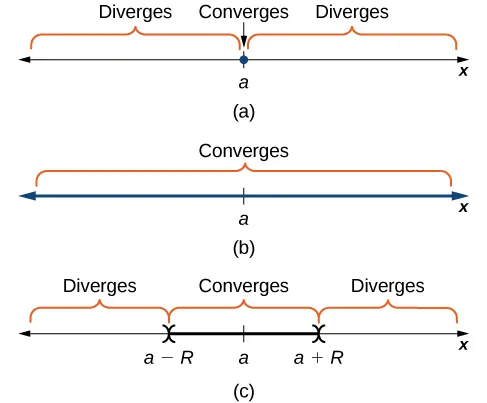
\includegraphics[scale=0.5]{./figures/popp.png}
    \end{center}

    \pagebreak \bigbreak \noindent 
    \begin{eg}
        Find the interval and radius of convergence
        \begin{align*}
            \summation{\infty}{n=1}\ \frac{x^{n}}{n!}\ 
        .\end{align*}
    \end{eg}
    \bigbreak \noindent 
    \textbf{Solution.} For this, we use the ratio test and get
    \begin{align*}
        &\rho = \lim\limits_{n \to \infty}{\bigg\lvert \frac{\frac{x^{n}\cdot x}{n!(n+1)}}{\frac{n!}{x^{n}}} \bigg\rvert} \\
        &=\abs{x}\lim\limits_{n \to \infty}{\frac{1}{n+1}} \\
        &=0
    .\end{align*}
    \bigbreak \noindent 
    Since $ 0 \leq \rho  < 1$, this series will converge $\fa x \in \mathbb{R} $. Thus, the interval of convergence is $(-\infty,+\infty) $ and the radius of convergence is $R = \infty $

    \bigbreak \noindent 
    \begin{eg}
         Find the interval and radius of convergence
         \begin{align*}
             \summation{\infty}{n=0}\ n!x^{n}\ 
         .\end{align*}
    \end{eg}
    \bigbreak \noindent 
    \textbf{Solution.} Again, we use the ratio test
    \begin{align*}
        &\rho = \lim\limits_{n \to \infty}{\frac{n!(n+1)x^{n}x}{n!x^{n}}} \\
        &=\abs{x}\lim\limits_{n \to \infty}{(n+1)} \\
        &=\infty
    .\end{align*}
    \bigbreak \noindent 
    Since $\rho = \infty $ The series diverges for all \( x \neq 0 \). Since the series is centered at \( x = 0 \), it must converge there, so the series converges only for \( x = 0 \). The interval of convergence is the single value \( x = 0 \) and the radius of convergence is \( R = 0 \).

    \pagebreak \bigbreak \noindent 
    \begin{eg}
        Find the interval and radius of convergence
        \begin{align*}
            \summation{\infty}{n=0}\ \frac{(x-2)^{n}}{(n+1)3^{n}}\ 
        .\end{align*}
    \end{eg}
    \bigbreak \noindent 
    \textbf{Solution.} After applying the ratio test, we get
    \begin{align*}
        &\rho = \abs{x-2}\lim\limits_{n \to \infty}{\frac{n+1}{3n+2}} \\
        &=\frac{\abs{x-2}}{3}
    .\end{align*}
    \bigbreak \noindent 
    The question we ask is... when is this quantity $<1 $. 
    \begin{align*}
        &\frac{\abs{x-2}}{3} < 1 \\
        &\abs{x-2} < 3 \\
        &\implies -3 < x-2 < 3 \\
        &-1 < x < 5
    .\end{align*}
    \bigbreak \noindent 
    Thus, when $-1 < x < 5$, the series will converge absolutely. Likewise
    \begin{align*}
        &\frac{\abs{x-2}}{3} > 1 \\
        &\abs{x-2} > 3 \\
        \implies &x-2 < -3 \quad \text{ or } x-2 > 3 \\
        &x < -1 \quad \text{ or } x > 5
    .\end{align*}
    \bigbreak \noindent 
    Thus, the series will diverge if $x < -1$ or $x > 5$. Finally, we examine if $\rho = 1$
    \begin{align*}
        \frac{\abs{x-2}}{3} &= 1 \\
        \abs{x-2} &= 3 \\
        x-2 = 3 \quad &\quad x-2 = -3 \\
        x=5 \quad &\quad x=-1
    .\end{align*}
    \bigbreak \noindent 
    Thus, the ratio test is inconclusive for $x = -1$ or $x=5$. We need to test these values of $x$ separately. For $x=-1$ the series is given by
    \begin{align*}
        &\summation{\infty}{n=0}\ \frac{(-3)^{n}}{(n+1)3^{n}}\  \\
        &=\summation{\infty}{n=0}\ \frac{3^{n}(-1)^{n}}{(n+1)3^{n}}\  \\
        &=\summation{\infty}{n=0}\ \frac{(-1)^{n}}{n+1}\  
    .\end{align*}
    \bigbreak \noindent 
    Since this is the alternating harmonic series, it converges. Thus, the series converges at  $x=-1$. For $x=5$, the series is given by
    \begin{align*}
        &\summation{\infty}{n=0}\ \frac{3^{n}}{(n+1)3^{n}}\  \\
        &\summation{\infty}{n=0}\ \frac{1}{n+1}\ 
    .\end{align*}
    This is the harmonic series, which is divergent. Therefore, the power series diverges at \( x = 5 \). We conclude that the interval of convergence is \([ -1, 5 )\) and the radius of convergence is \( R = 3 \).

    \bigbreak \noindent 
    \phantomsection
    \addcontentsline{toc}{subsection}{Representing Functions as Power Series}
    \subsection*{Representing Functions as Power Series}
    \bigbreak \noindent 
    Being able to represent a function by an “infinite polynomial” is a powerful tool. Polynomial functions are the easiest functions to analyze, since they only involve the basic arithmetic operations of addition, subtraction, multiplication, and division. If we can represent a complicated function by an infinite polynomial, we can use the polynomial representation to differentiate or integrate it. In addition, we can use a truncated version of the polynomial expression to approximate values of the function. So, the question is, when can we represent a function by a power series?
    \bigbreak \noindent 
    Consider again the geometric series
\begin{equation}
    1 + x + x^2 + x^3 + \cdots = \sum_{n=0}^{\infty} x^n 
\end{equation}
Recall that the geometric series
\[
    a + ar + ar^2 + ar^3 + \cdots
\]
converges if and only if \( |r| < 1 \). In that case, it converges to \(\frac{a}{1 - r}\). Therefore, if \( |x| < 1 \), the series in Example 6.3 converges to \(\frac{1}{1 - x}\) and we write
\[
    1 + x + x^2 + x^3 + \cdots = \frac{1}{1 - x} \quad \text{for} \quad |x| < 1.
\]
As a result, we are able to represent the function \( f(x) = \frac{1}{1 - x} \) by the power series
\[
    1 + x + x^2 + x^3 + \cdots \quad \text{when} \quad |x| < 1.
\]
We now show graphically how this series provides a representation for the function \( f(x) = \frac{1}{1 - x} \) by comparing the graph of \( f \) with the graphs of several of the partial sums of this infinite series.

    \bigbreak \noindent 
    \begin{eg}
       Use a power series to represent each of the following functions  $f$. Find the interval of convergence. 
       \begin{align*}
           f(x) = \frac{1}{1+x^{3}}
       .\end{align*}
    \end{eg}
    \bigbreak \noindent 
    \textbf{Solution.} should recognize this function $f$ as the sum of a geometric series, because
    \begin{align*}
        \frac{1}{1+x^{3}} = \frac{1}{1-(-x^{3})}
    .\end{align*}
    Using the fact that, for \( |r| < 1 \), \(\frac{a}{1 - r}\) is the sum of the geometric series
\[
    \sum_{n=0}^{\infty} ar^n = a + ar + ar^2 + \cdots,
\]
we see that, for \( \left| -x^3 \right| < 1 \),
\[
    \frac{1}{1 + x^3} = \frac{1}{1 - (-x^3)} = \sum_{n=0}^{\infty} (-x^3)^n = 1 - x^3 + x^6 - x^9 + \cdots.
\]
Since this series converges if and only if \( \left| -x^3 \right| < 1 \), the interval of convergence is \( (-1, 1) \), and we have
\[
    \frac{1}{1 + x^3} = 1 - x^3 + x^6 - x^9 + \cdots \quad \text{for} \quad |x| < 1.
\]


    \pagebreak \bigbreak \noindent 
    \begin{eg}
       Use a power series to represent each of the following functions  $f$. Find the interval of convergence. 
       \begin{align*}
           \summation{\infty}{n=0}\ \frac{x^{2}}{4-x^{2}}\ 
       .\end{align*}
    \end{eg}
    \bigbreak \noindent 
    This function is not in the exact form of a sum of a geometric series. However, with a little algebraic manipulation, we can relate \( f \) to a geometric series. By factoring \( 4 \) out of the two terms in the denominator, we obtain
    \[
        \frac{x^2}{4 - x^2} = \frac{x^2}{4(1 - \frac{x^2}{4})} = \frac{x^2}{4}\left(1 - \left(\frac{x^2}{2}\right)^2\right).
    \]
    \bigbreak \noindent 
    Therefore, we have
    \[
        \frac{x^2}{4 - x^2} = \frac{x^2}{4}\left(1 - \left(\frac{x^2}{2}\right)^2\right) = \frac{x^2}{4}\frac{1}{1 - \left(\frac{x^2}{2}\right)^2} = \sum_{n=0}^{\infty} \frac{x^2}{4}\left(\frac{x^2}{2}\right)^{2n}.
    \]
    \bigbreak \noindent 
    The series converges as long as \( \left|\left(\frac{x^2}{2}\right)^2\right| < 1 \) (note that when \( \left|\left(\frac{x^2}{2}\right)^2\right| = 1 \) the series does not converge). Solving this inequality, we conclude that the interval of convergence is \( (-2, 2) \), and
    \[
        \frac{x^2}{4 - x^2} = \sum_{n=0}^{\infty} \frac{x^{2n?2}}{4^{n+1}} = \frac{x^2}{4} + \frac{x^4}{4^2} + \frac{x^6}{4^3} + \cdots
    \]
    \bigbreak \noindent 
    for \( |x| < 2 \).

        
        


    


    
    
    
    


\end{document}
